% Options for packages loaded elsewhere
\PassOptionsToPackage{unicode}{hyperref}
\PassOptionsToPackage{hyphens}{url}
%
\documentclass[
]{article}
\usepackage{amsmath,amssymb}
\usepackage{iftex}
\ifPDFTeX
  \usepackage[T1]{fontenc}
  \usepackage[utf8]{inputenc}
  \usepackage{textcomp} % provide euro and other symbols
\else % if luatex or xetex
  \usepackage{unicode-math} % this also loads fontspec
  \defaultfontfeatures{Scale=MatchLowercase}
  \defaultfontfeatures[\rmfamily]{Ligatures=TeX,Scale=1}
\fi
\usepackage{lmodern}
\ifPDFTeX\else
  % xetex/luatex font selection
\fi
% Use upquote if available, for straight quotes in verbatim environments
\IfFileExists{upquote.sty}{\usepackage{upquote}}{}
\IfFileExists{microtype.sty}{% use microtype if available
  \usepackage[]{microtype}
  \UseMicrotypeSet[protrusion]{basicmath} % disable protrusion for tt fonts
}{}
\makeatletter
\@ifundefined{KOMAClassName}{% if non-KOMA class
  \IfFileExists{parskip.sty}{%
    \usepackage{parskip}
  }{% else
    \setlength{\parindent}{0pt}
    \setlength{\parskip}{6pt plus 2pt minus 1pt}}
}{% if KOMA class
  \KOMAoptions{parskip=half}}
\makeatother
\usepackage{xcolor}
\usepackage[margin=1in]{geometry}
\usepackage{longtable,booktabs,array}
\usepackage{calc} % for calculating minipage widths
% Correct order of tables after \paragraph or \subparagraph
\usepackage{etoolbox}
\makeatletter
\patchcmd\longtable{\par}{\if@noskipsec\mbox{}\fi\par}{}{}
\makeatother
% Allow footnotes in longtable head/foot
\IfFileExists{footnotehyper.sty}{\usepackage{footnotehyper}}{\usepackage{footnote}}
\makesavenoteenv{longtable}
\usepackage{graphicx}
\makeatletter
\def\maxwidth{\ifdim\Gin@nat@width>\linewidth\linewidth\else\Gin@nat@width\fi}
\def\maxheight{\ifdim\Gin@nat@height>\textheight\textheight\else\Gin@nat@height\fi}
\makeatother
% Scale images if necessary, so that they will not overflow the page
% margins by default, and it is still possible to overwrite the defaults
% using explicit options in \includegraphics[width, height, ...]{}
\setkeys{Gin}{width=\maxwidth,height=\maxheight,keepaspectratio}
% Set default figure placement to htbp
\makeatletter
\def\fps@figure{htbp}
\makeatother
\setlength{\emergencystretch}{3em} % prevent overfull lines
\providecommand{\tightlist}{%
  \setlength{\itemsep}{0pt}\setlength{\parskip}{0pt}}
\setcounter{secnumdepth}{5}
\usepackage{booktabs}
\usepackage{longtable}
\usepackage{array}
\usepackage{multirow}
\usepackage{wrapfig}
\usepackage{float}
\usepackage{colortbl}
\usepackage{pdflscape}
\usepackage{tabu}
\usepackage{threeparttable}
\usepackage{threeparttablex}
\usepackage[normalem]{ulem}
\usepackage{makecell}
\usepackage{xcolor}
\ifLuaTeX
  \usepackage{selnolig}  % disable illegal ligatures
\fi
\IfFileExists{bookmark.sty}{\usepackage{bookmark}}{\usepackage{hyperref}}
\IfFileExists{xurl.sty}{\usepackage{xurl}}{} % add URL line breaks if available
\urlstyle{same}
\hypersetup{
  pdftitle={BauchRhoMFig},
  pdfauthor={Sophie Wulfing},
  hidelinks,
  pdfcreator={LaTeX via pandoc}}

\title{BauchRhoMFig}
\author{Sophie Wulfing}
\date{30 September, 2023, 13:00}

\begin{document}
\maketitle

\begin{figure}
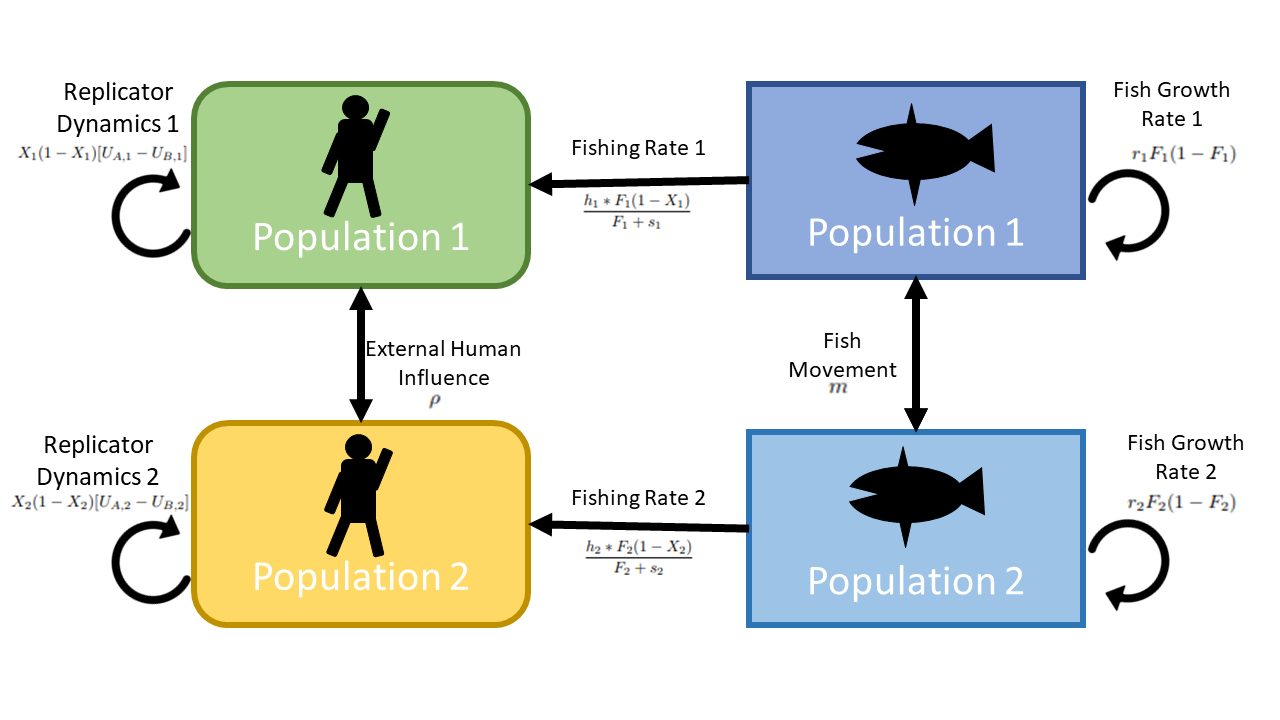
\includegraphics[width=1\linewidth]{CoupledModelConceptual} \caption{A conceptual representation of our model as a two-patch extension of @bauchEarlyWarningSignals2016. Here, each fish population (\(F_i\)) in each patch \(i\) increase through natural growth and movement of fish into the patch. Fish populations are decreased through emigration out of the patch and fishing mortality. The number of fishers (\(X_i\)) in each patch \(i\) change in response to fish population levels, the cost of stopping fishing activity, and the opinions of those in the patch and those in the other patch. \label{Conceptual}}\label{fig:Conceptual}
\end{figure}



\begin{table}

\caption{\label{tab:paramtable}Parameter values used in this analysis. Taken from Bauch et al appendix where oscillations are observed. DOUBLE CHECK THAT}
\centering
\begin{tabular}[t]{llll}
\toprule
Parameter & Population\_1 & Population\_2 & Def\\
\midrule
r & 0.16 & 0.16 & Fish net growth\\
s & 0.8 & 0.8 & Supply and demand\\
h & 0.25 & 0.25 & Harvesting efficiency\\
k & 0.17 & 0.17 & Social learning rate\\
w & 1.44 & 1.44 & Conservation cost\\
\addlinespace
c & 0.5 & 0.5 & Rarity valuation\\
d & 0.3 & 0.3 & Social norm strength (within pop)\\
m & 0 & 0 & Fish movement (from opposite patch)\\
rho & 0 & 0 & Social norm strength (opposite pop)\\
\bottomrule
\end{tabular}
\end{table}

\begin{figure}
\centering
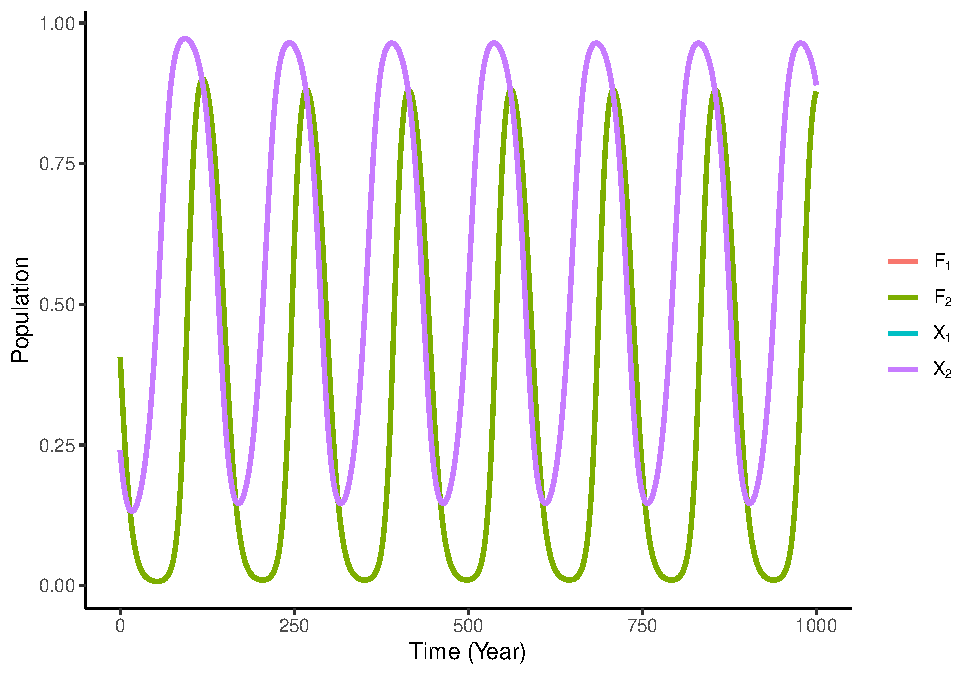
\includegraphics{SubmissionFigs_files/figure-latex/Bauch.Coupled-1.pdf}
\caption{(\#fig:Bauch.Coupled)New Model with default paramters given in Bauch et al.~Demonstrating homogenous populations.}
\end{figure}

\hypertarget{movement}{%
\section{MOVEMENT}\label{movement}}

\begin{figure}
\centering
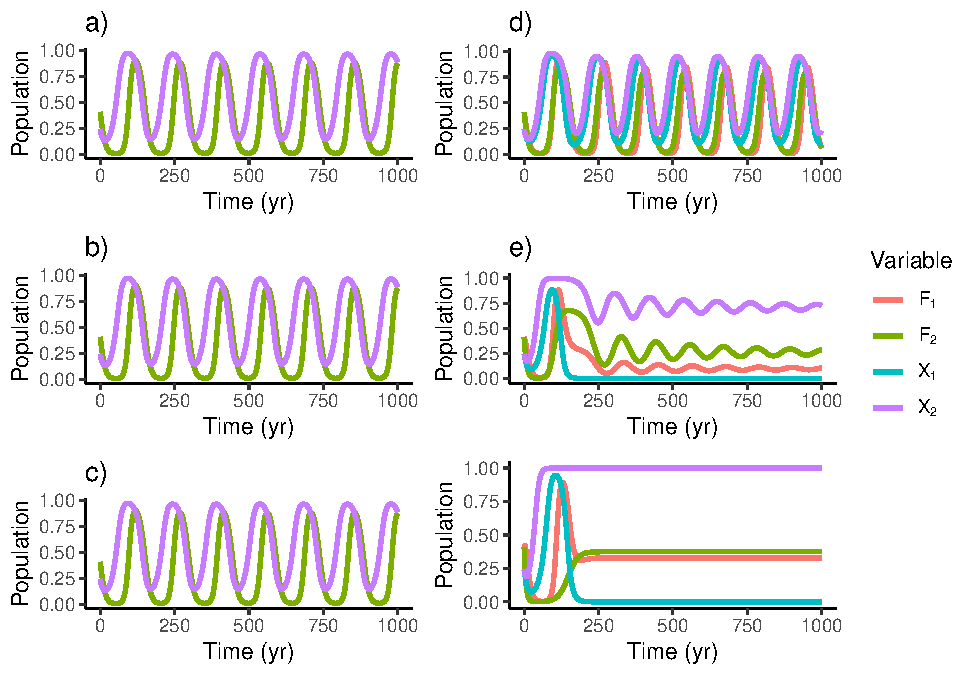
\includegraphics{SubmissionFigs_files/figure-latex/movement-1.pdf}
\caption{\label{fig:movement}Showing that movement only matters when there is asymmetry. This can be asymmetry in other params. When this is the case, high movement dampens oscillatory effects}
\end{figure}

\begin{figure}
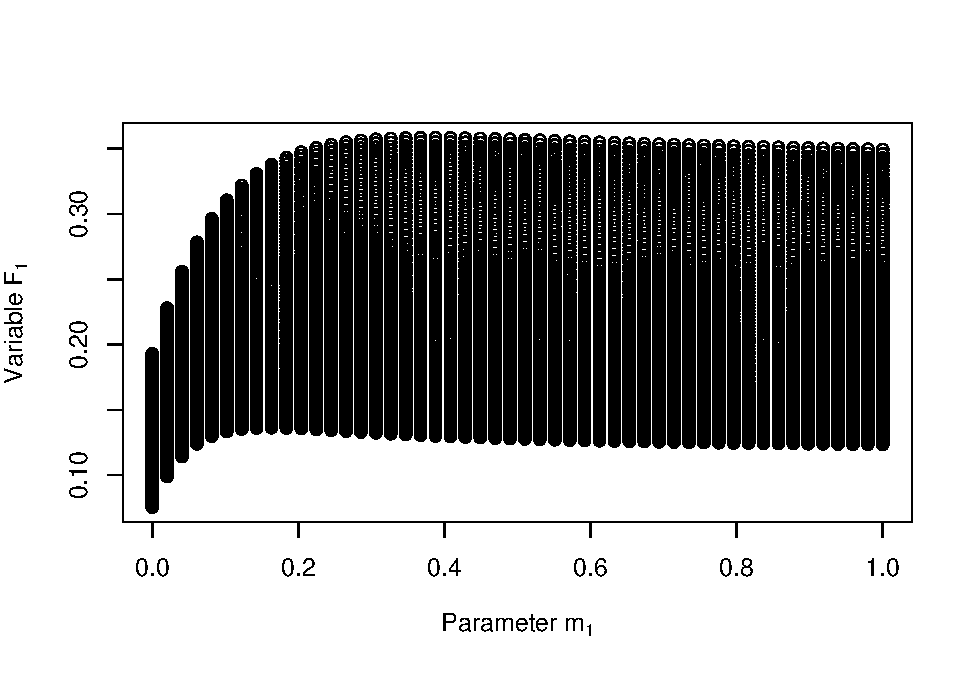
\includegraphics[width=0.5\linewidth]{SubmissionFigs_files/figure-latex/mBifCurve-1} 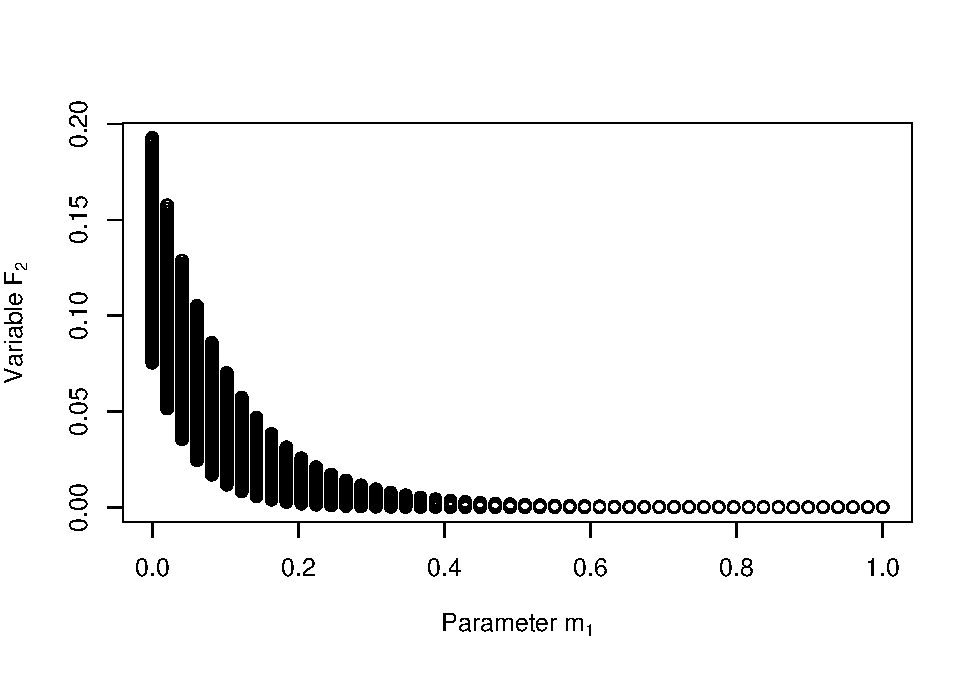
\includegraphics[width=0.5\linewidth]{SubmissionFigs_files/figure-latex/mBifCurve-2} \caption{Bifurcation curves of fish pops in response to changes in m1 paramter. Shows how high m parameters eliminates oscillations.}\label{fig:mBifCurve}
\end{figure}

\hypertarget{social-influence-stuff}{%
\section{SOCIAL INFLUENCE STUFF}\label{social-influence-stuff}}



\begin{figure}
\centering
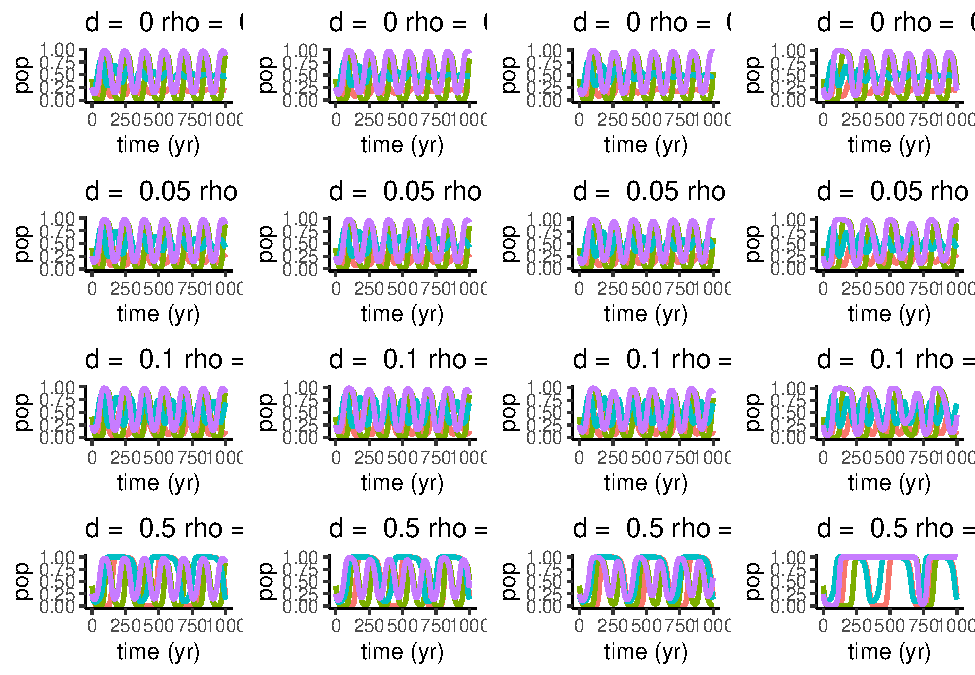
\includegraphics{SubmissionFigs_files/figure-latex/influenceAsym-1.pdf}
\caption{\label{fig:influenceAsym}This shows the difference between a pop 1 listening to themselves vs.~other pop. Looking at red line (which is fish in pop 1), this demonstrates that a portfolio effect can smooth over variation in dynamics. See how red line levels out when rho is high but with a low d.~high d and low rho results in high fluctuations in stocks \label{influenceAsym}}
\end{figure}

\hypertarget{scenarios}{%
\section{SCENARIOS}\label{scenarios}}



\begin{longtable}[]{@{}llll@{}}
\caption{\label{tab:DispersionParamTable}Parameter values used to simulate sustainable fishing practices in patch 1 and overfishing in patch 2. \label{DispersionParamTable}}\tabularnewline
\toprule\noalign{}
Parameter & Population 1 & Population 2 & Definition \\
\midrule\noalign{}
\endfirsthead
\toprule\noalign{}
Parameter & Population 1 & Population 2 & Definition \\
\midrule\noalign{}
\endhead
\bottomrule\noalign{}
\endlastfoot
r & 0.4 & 0.35 & Fish net growth \\
s & 0.8 & 0.8 & Supply and demand \\
h & 0.25 & 0.5 & Harvesting efficiency \\
k & 1.014 & 1.014 & Rate of sampling opinions or social interaction \\
\(\omega\) & 0.2 & 0.35 & Conservation cost \\
c & 1.5 & 1.5 & Rarity valuation \\
d & 0.5 & 0.5 & Strength of social influence (within population) \\
m & 0.2 & 0.2 & Fish movement (from opposite patch) \\
\(\rho\) & 0.5 & 0.1 & Strength of social influence (opposite population) \\
\end{longtable}



\begin{figure}
\centering
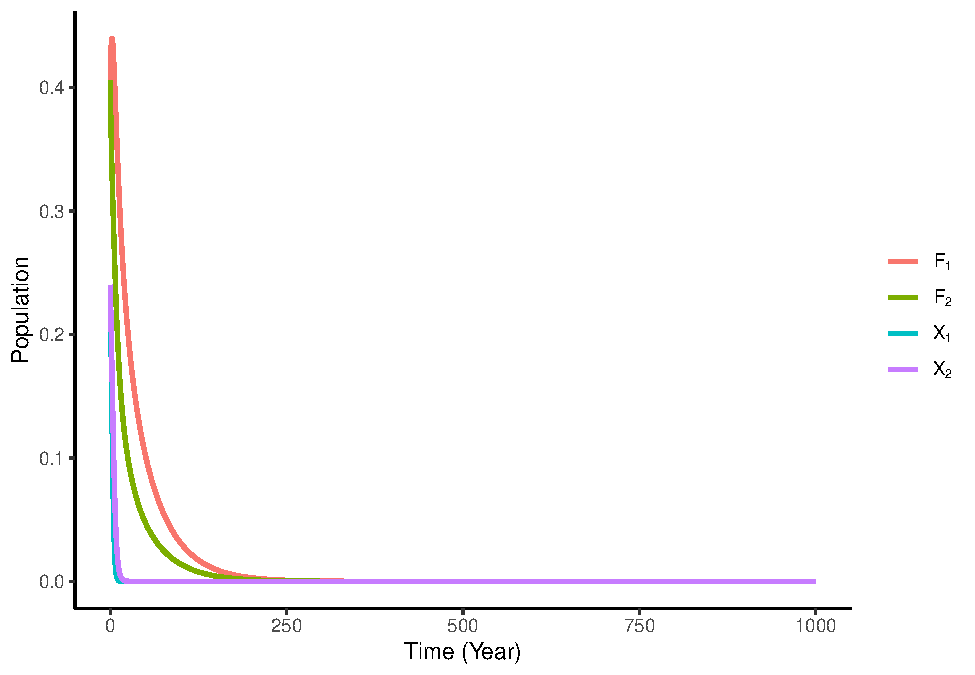
\includegraphics{SubmissionFigs_files/figure-latex/DispersionScenario-1.pdf}
\caption{\label{fig:DispersionScenario}Representation of the dynamics of both the fish populations (\(F_i\)) and human conservationists (\(X_i\)) in each patch with default parameters from table \ref{DispersionParamTable} after 1000 years. This just shows how the unsustainable fishing results in the whole thing collapsing \label{DispersionScenario}}
\end{figure}



\begin{figure}
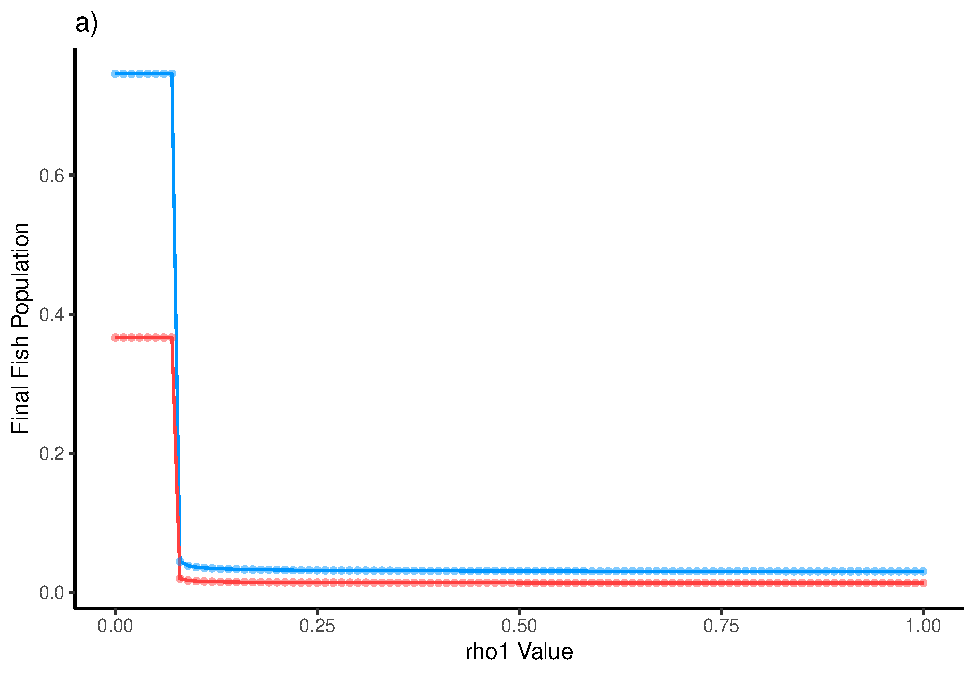
\includegraphics[width=0.5\linewidth]{SubmissionFigs_files/figure-latex/rhoExploreGraphEach-1} 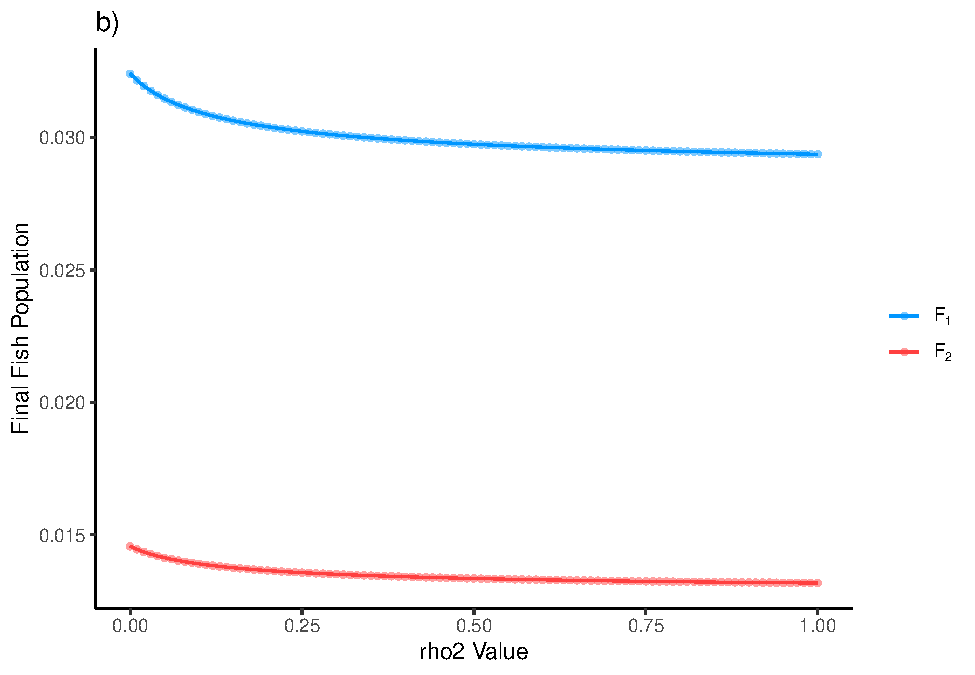
\includegraphics[width=0.5\linewidth]{SubmissionFigs_files/figure-latex/rhoExploreGraphEach-2} \caption{Each rho individually. Ok so here's my confusion, above in \ref:influenceasym I say that incorporating new information will increase stability but here, as pop 2 (which is unsustainable) listens to pop 1 more, the whole thing crashes. Earlier we said this was because pop 1 is continuing to fish, so therefore encouraging pop 2 to fish more (looking at graph a) \label{rhoExploreGraphEach}}\label{fig:rhoExploreGraphEach}
\end{figure}



\begin{figure}
\centering
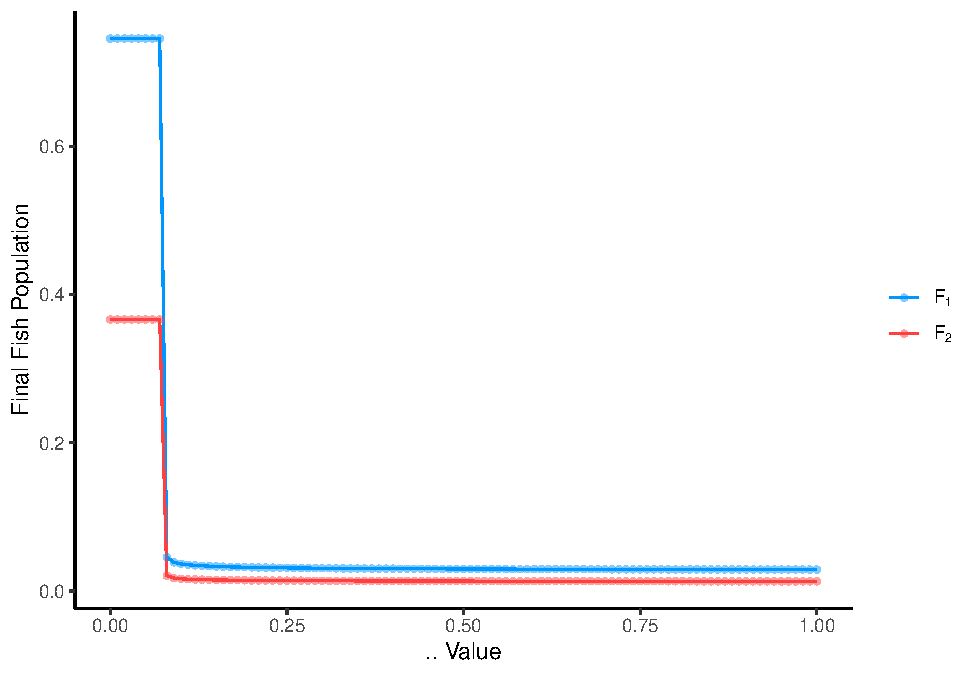
\includegraphics{SubmissionFigs_files/figure-latex/rhoExploreGraph-1.pdf}
\caption{\label{fig:rhoExploreGraph}Final fish populations after 100 years in the two-patch fishing model where the \(F_1\) population in patch 1 is fished sustainably but human population 1 has a lower social influence than humans in patch 2, where \(F_2\) is being fished unsustainably. Both \(\rho_1\) and \(\rho_2\) were increased simultaneously. \label{rhoExploreGraph}}
\end{figure}



\begin{figure}
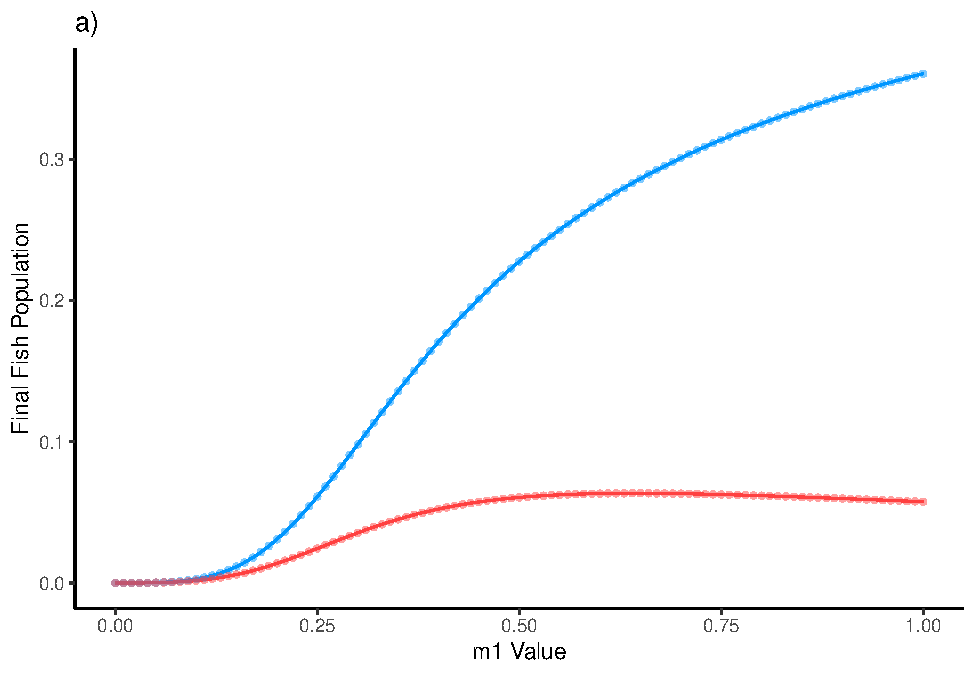
\includegraphics[width=0.5\linewidth]{SubmissionFigs_files/figure-latex/mExploreGraph-1} 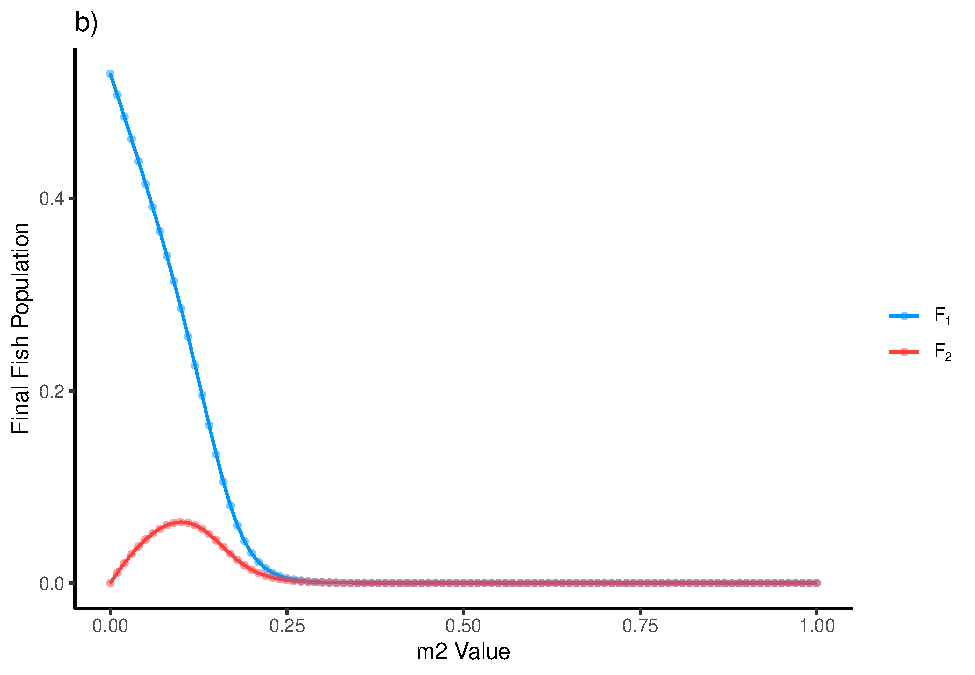
\includegraphics[width=0.5\linewidth]{SubmissionFigs_files/figure-latex/mExploreGraph-2} \caption{Final fish populations after 100 years in the two-patch fishing model where patch 1 (\(F_1\)) is fished sustainably but human population 1 has a lower social influence than patch 2, where \(F_2\) is being fished unsustainably. a) shows how increases in fish movement into patch 1 (\(m_1\)) affect final populations and b) shows how increases in fish movement into patch 2 (\(m_2\)) affect final populations. More fish moving to sustainable patch (a). Will result in both grousps increasing fish. Showing how one patch CAN save whole system if enough fish are subject to their fishing. b) shows how if more fish move to unsustained patch, whole system will crash. \label{mExploreGraph}}\label{fig:mExploreGraph}
\end{figure}



\begin{figure}
\centering
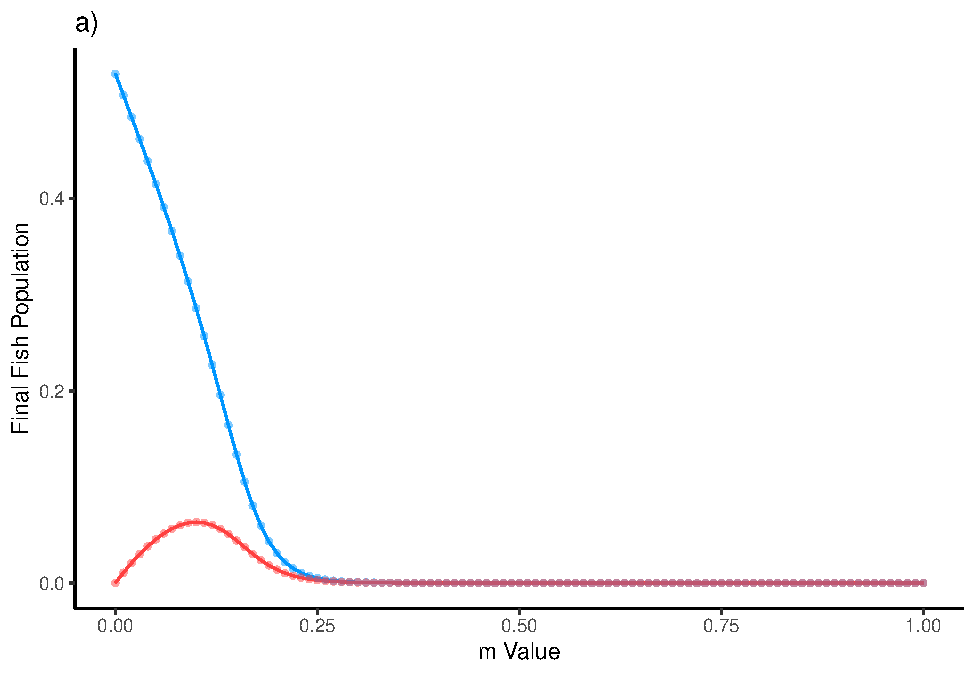
\includegraphics{SubmissionFigs_files/figure-latex/mExploreGraphBoth-1.pdf}
\caption{\label{fig:mExploreGraphBoth}Both ms changing. Increasing both ms results in fishery crashes. Probably due to more fish entering F2 to be overfished more? \label{mExploreGraphBoth}}
\end{figure}

\hypertarget{appendix-stuff}{%
\section{APPENDIX STUFF}\label{appendix-stuff}}

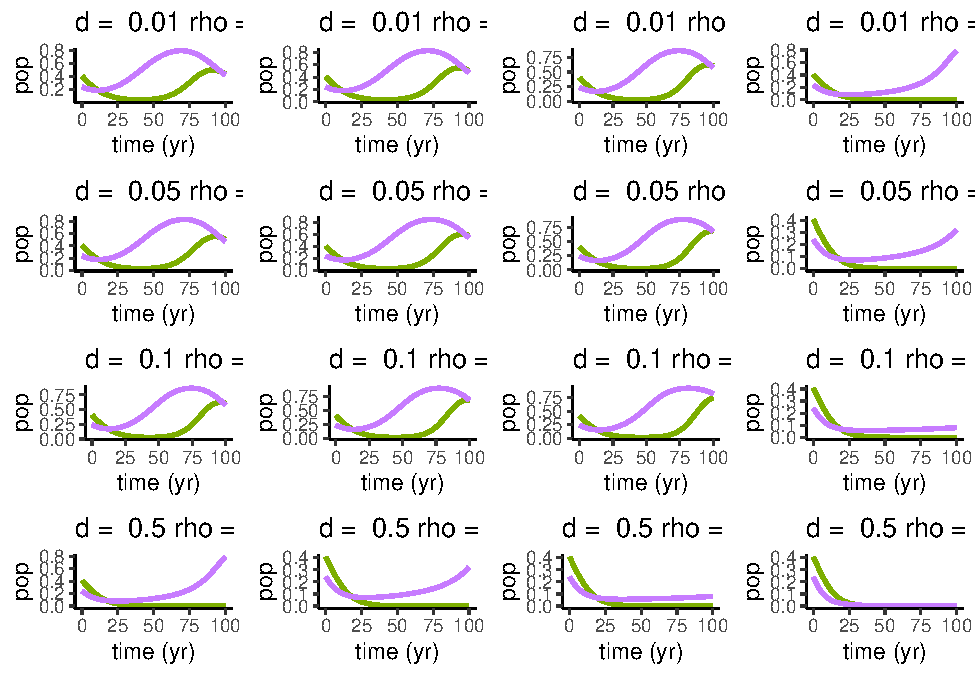
\includegraphics{SubmissionFigs_files/figure-latex/influenceBoth-1.pdf}
Essentially shows that with symmetry, d and rho act similarly. When one or the other is strong, you get delayed cycles (i.e.~delayed reactions to pressure)

\end{document}
